\documentclass{article}

% --- load packages ---
\usepackage[margin=1in]{geometry} % change the margins
\usepackage{amsmath} % useful math environments and commands like align
\usepackage[colorlinks,bookmarks,bookmarksnumbered,allcolors=blue]{hyperref} % hyperlinks between references
\usepackage{graphicx}  % include images
\usepackage[table,xcdraw]{xcolor}
\usepackage[caption=false]{subfig} % subfigures.  false option prevents conflicts in caption styling with other packages
\usepackage{booktabs} % better tables
\usepackage[capitalise]{cleveref} % better referencing. uses cref.
\usepackage[section]{placeins} % sometimes useful to prevent figures from floating out of a section
\usepackage{cite} % handles multiple citations in one command better
\usepackage{doi} % allow correct hypderlinking of DOIs
\usepackage[normalem]{ulem}
\usepackage{float}
\usepackage{minted}
\usepackage{pdfpages}
\usepackage{tikz}
\usetikzlibrary{tikzmark}


%\usepackage{lmodern}

\useunder{\uline}{\ul}{}
\newcommand{\test}{Here is the test text to display}


\begin{document}

\title{Unconstrained Optimization}
\author{Landon Wright}
% put in \date{} if you don't want a date to appear, or enter a specific date, otherwise default is today's date.
\maketitle
\section{Program Description}
\section{Testing Results}
\subsection{Function 1 Results}
% Steepest descent data

% Conjugate gradient data

% BFGS quasi-Newton data

% table of obj evals and gradient evals for each method
\subsection{Rosenbrock Function Results}
% plot for steepest descent

% plot for conjugate gradient

% plot for quasi-Newton

% table of obj and gradient evals for each method


\section{Matlab Code}

\subsection{Fminun Routine}
\inputminted[xleftmargin=20pt,linenos]{matlab}{fminun.m}
\subsection{Alpha\_star line search}
\inputminted[xleftmargin=20pt, linenos]{matlab}{aPrime.m}
\subsection{Driver}
\inputminted[xleftmargin=20pt,linenos]{matlab}{fminunDriv.m}

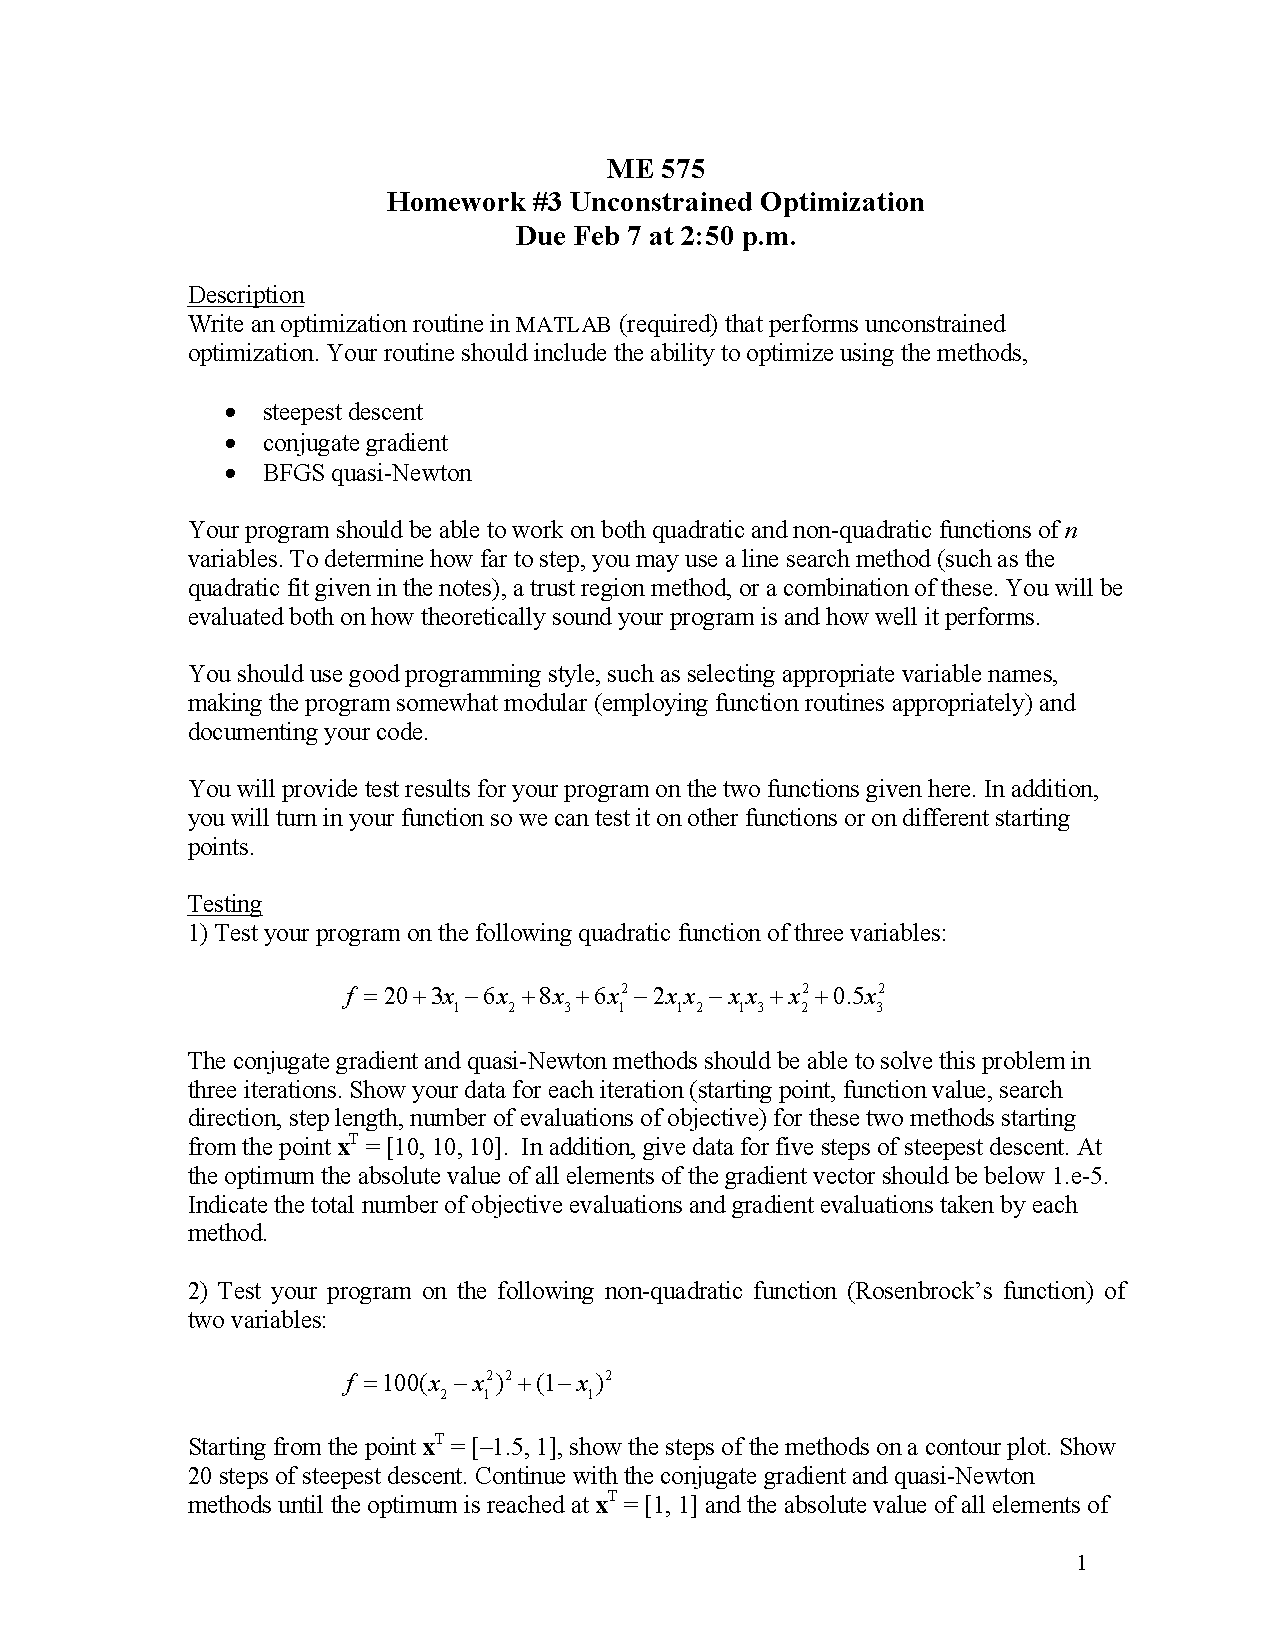
\includepdf[pages=-, pagecommand={}]{HW3Unconstrained.pdf}
\end{document}
